\subsection{UC-19}
\label{subsec:UC-19}

\begin{figure}[H]
    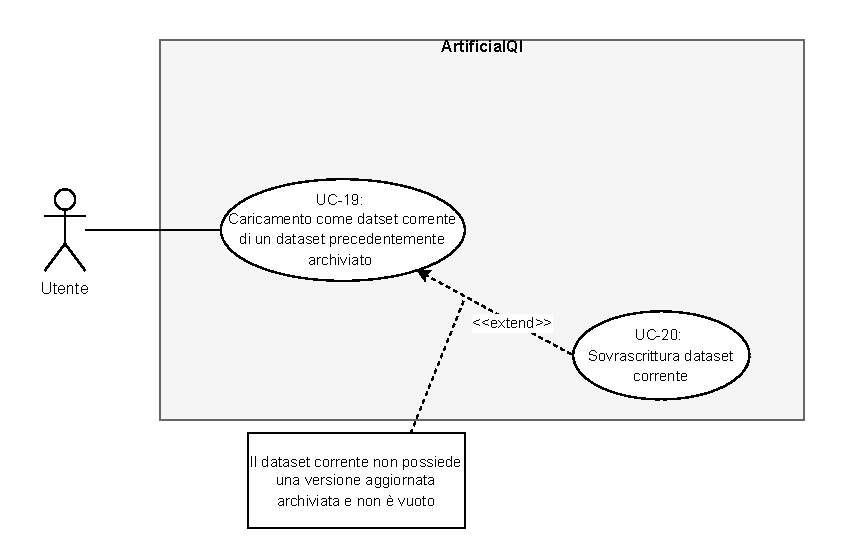
\includegraphics{Sezioni/UseCase/Immagini/UC-19.pdf}
    \caption{Diagramma UC-19.}
\end{figure}

\begin{usecase}{UC-19}{Caricamento come dataset corrente di un dataset archiviato}

    \req{\hyperref[item:RU-6]{RU-6}} 

    \pre{
        \item Il sistema è attivo e funzionante
        \item Il dataset da caricare come dataset corrente è stato precedentemente archiviato
    }

    \post{
        \item Il dataset viene caricato come dataset corrente
    }
    
    \actor{Utente}

    \subactors{}

    \trigger{L'utente deve caricare come dataset corrente uno tra quelli archiviati}
    
    \inc{}

    \base{}

    \scenario{
        \item L'utente richiede di caricare un dataset archiviato
        \item Il dataset scelto viene caricato come dataset corrente
    }

    \subscenario{
        \item[2.1] \textbf{Il dataset caricato non possiede una versione aggiornata archiviata e non è vuoto}
        \begin{itemize}
            \item[a.] \hyperref[subsec:UC-20]{UC-20}
        \end{itemize}
    }
\end{usecase}